\section{Projektmanagement}
Das Modul PREN ist ein interdisziplinäres Modul. Von jeder der Fachrichtungen 
Informatik, Elektrotechnik und Maschinenbau ist mindestens eine Person pro 
Gruppe vertreten. Das Team 27 setzt sich wie folgt zusammen:
\begin{itemize}
    \item 3 Informatiker
    \item 3 Maschinenbauer
    \item 1 Elektrotechniker
\end{itemize}
Zu Beginn des Moduls wurden den Mitgliedern des Teams verschiedene Funktionen 
zugewiesen, um eine Struktur und somit Ansprechpersonen innerhalb des Teams zu 
erhalten. Ersichtlich ist dies in folgendem Organigramm:
\newcommand\orgnode[6][]{
    \node[#1] at (#2) {
        \boxed{
            \parbox{40pt} {%
                \includegraphics[width=40pt]{#3}}%
            \parbox{10pt}{\mbox{}}%  
            \parbox{\dimexpr4.0cm-30pt\relax}{
                \textbf{#4}\\
                [.4ex]\textit{#5}\\
                [.4ex]#6\\}%
        }
    };
}
\begin{figure}[h!]
    % from http://tex.stackexchange.com/questions/170154/organisation-chart-in-latex-using-tikz
    \centering
    \begin{tikzpicture}
        \orgnode
            {0,0}
            {../fig/takuonen.png}
            {Peter Kuonen}
            {Informatik}
            {Projektleiter}
        \orgnode
            {-6,-4}
            {../fig/tawinz.png}
            {Daniel Winz}
            {Elektrotechnik}
            {Bereichsleiter E}
        \orgnode
            {0,-4}
            {../fig/mamaisse.png}
            {Andriu Maissen}
            {Maschinenbau}
            {Bereichsleiter M}
        \orgnode
            {6,-4}
            {../fig/taneidha.png}
            {Simon Neidhart}
            {Informatik}
            {Bereichsleiter I}
        \orgnode
            {0,-8}
            {../fig/tfkueng.png}
            {Yannik Küng}
            {Maschinenbau}
            {Projektmitarbeiter}
        \orgnode
            {0,-12}
            {../fig/tfmathis.png}
            {Daniel Mathis}
            {Maschinenbau}
            {Projektmitarbeiter}
        \orgnode
            {6,-8}
            {../fig/tcwespi.png}
            {Kevin Wespi}
            {Informatik}
            {Protokollführer}
        \draw[-latex, thick] (0,-1) -- (0,-2) -- (-6,-2) -- (-6,-3);
        \draw[-latex, thick] (0,-1) -- (0,-2) -- (0,-2) -- (0,-3);
        \draw[-latex, thick] (0,-1) -- (0,-2) -- (6,-2) -- (6,-3);
        \draw[-latex, thick] (-2.4,-4) -- (-2.9,-4) -- (-2.9,-8) -- (-2.4, -8);
        \draw[-latex, thick] (-2.4,-4) -- (-2.9,-4) -- (-2.9,-12) -- (-2.4, -12);
        \draw[-latex, thick] (3.6,-4) -- (3.1,-4) -- (3.1,-8) -- (3.6, -8);
    \end{tikzpicture}
    \caption{Organigramm}
    \label{fig:Organigramm}
\end{figure}

\subsection{Projektplanung}
In den folgenden Abbildungen wird die Planung mittels Zeitachsen für die 
einzelnen Meilensteine dargestellt. Sie enthalten die Hauptaufgaben, welche 
für die jeweiligen Meilensteine notwendig sind. Die Planung wird angefertigt 
um die Übersicht über das Projekt zu haben und die verlangten Dokumente und 
Schritte zur Erfüllung der Meilensteine fristgerecht zu erledigen.

\begin{figure}[h!]
    \centering
    \begin{tikzpicture}[scale=0.5]
        % Phases
        \draw[fill=lgray, align=center, rounded corners] (0,- 0) rectangle node {Moduleinführung\\Teambildung\\Projektinitialisierung} (-8,- 8);
        \draw[fill=lgray, align=center, rounded corners] (0,- 8) rectangle node {Projektplanung\\Anforderungen\\Recherche} (-8,-15);
        \draw[fill=lgray, align=center, rounded corners] (0,-15) rectangle node {Anforderungen\\Recherche} (-8,-22);
        % Days
        \draw[thick] (0,- 0) -- (1,- 0) node[right] {18.09.2014};
        \draw[thick] (0,- 1) -- (1,- 1) node[right] {19.09.2014};
        \draw[thick] (0,- 7) -- (1,- 7) node[right] {25.09.2014};
        \draw[thick] (0,- 8) -- (1,- 8) node[right] {26.09.2014};
        \draw[thick] (0,-14) -- (1,-14) node[right] {02.10.2014};
        \draw[thick] (0,-15) -- (1,-15) node[right] {03.10.2014};
        \draw[thick] (0,-21) -- (1,-21) node[right] {09.10.2014};
        \draw[thick] (0,-22) -- (1,-22) node[right] {10.10.2014};
        % Arrow
        \draw[line width=4, ->] (0,0) -- (0,-22.5);
    \end{tikzpicture}
    \caption{Planung Meilenstein 1 (Initialisierungsphase)}
    \label{fig:MS1}
\end{figure}
\begin{figure}[h!]
    \centering
    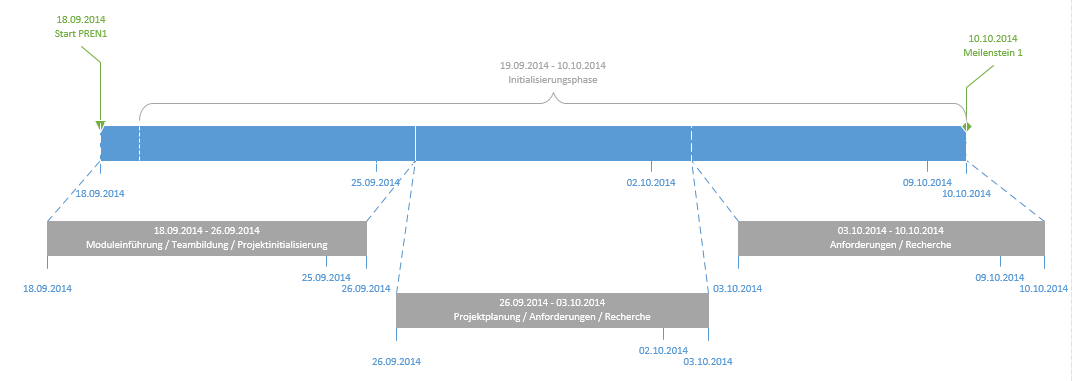
\includegraphics[angle=90,height=0.9\textheight]{fig/PlanungBisMS1.png}
    \caption{Planung Meilenstein 1}
    \label{fig:MS1}
\end{figure}
\begin{figure}[h!]
    \centering
    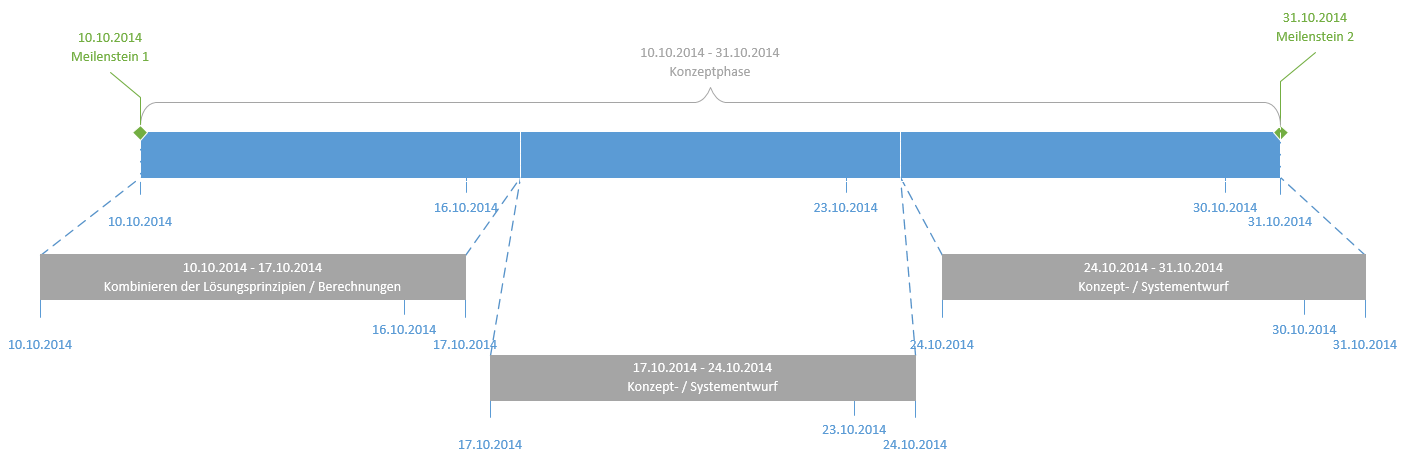
\includegraphics[angle=90,height=0.9\textheight]{fig/PlanungBisMS2.png}
    \caption{Planung Meilenstein 2}
    \label{fig:MS2}
\end{figure}
\begin{figure}[h!]
    \centering
    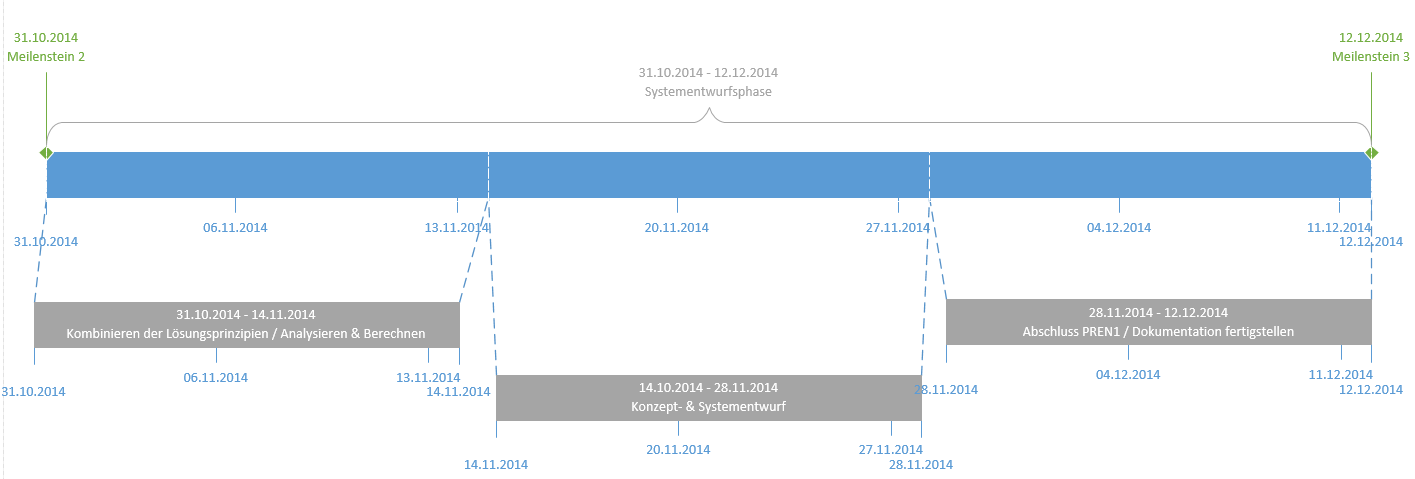
\includegraphics[angle=90,height=0.9\textheight]{fig/PlanungBisMS3.png}
    \caption{Planung Meilenstein 3}
    \label{fig:MS3}
\end{figure}
